\documentclass[12pt,a4paper]{article}
\usepackage[utf8]{inputenc}
\usepackage[a4paper,vmargin={17mm,20mm},hmargin={20mm,10mm}]{geometry}
\usepackage{amsmath}
\usepackage{amssymb}
\usepackage{mathtools}
\usepackage{gensymb}
\usepackage{enumitem}
\usepackage{graphicx}
\usepackage{scrextend}
\usepackage{blindtext}
\usepackage{caption}
% \usepackage{url}
\usepackage{hyperref}
\usepackage{subcaption}
\usepackage{circuitikz}
\usepackage{listings}
\usepackage{color}

\usepackage{xeCJK}
% \usepackage[UTF8]{ctex}
\usepackage{indentfirst}
% \usepackage[T1]{fontenc}
\usepackage{tgbonum}
\usepackage{float}

% 處理中文換行
\XeTeXlinebreaklocale "zh"
\XeTeXlinebreakskip = 0pt plus 1pt
%字體設定
% \setCJKmainfont[AutoFakeBold,AutoFakeSlant]{DFKai-SB}
\setCJKmainfont{Noto Serif CJK SC}
\setCJKmonofont{Noto Serif CJK SC}
% \setmainfont{Times New Roman}
% \fontfamily{ptm}
 
\definecolor{codegreen}{rgb}{0,0.6,0}
\definecolor{codegray}{rgb}{0.5,0.5,0.5}
\definecolor{codepurple}{rgb}{0.58,0,0.82}
\definecolor{backcolour}{rgb}{0.95,0.95,0.92}

\hypersetup{
    colorlinks=true,
    linkcolor=blue,
    filecolor=magenta,      
    urlcolor=cyan,
    % pdftitle={Overleaf Example},
    % pdfpagemode=FullScreen,
}
 
\lstdefinestyle{mystyle}{
    backgroundcolor=\color{backcolour},   
    commentstyle=\color{codegreen},
    keywordstyle=\color{magenta},
    numberstyle=\tiny\color{codegray},
    stringstyle=\color{codepurple},
    basicstyle=\ttfamily\footnotesize,
    breakatwhitespace=false,         
    breaklines=true,                 
    captionpos=b,                    
    keepspaces=true,                 
    numbers=left,                    
    numbersep=5pt,                  
    showspaces=false,                
    showstringspaces=false,
    showtabs=false,                  
    tabsize=2
}

\lstset{style=mystyle}
\setlength\parindent{2em}
% \parindent = 2em
% \setlength{\parskip}{-20pt}

\renewcommand{\lstlistingname}{Code}

\linespread{1.5}

\DeclarePairedDelimiter\floor{\lfloor}{\rfloor}
\title{Introduction to Computer Final Project Report}
\date{\today}
\author{By B11902006 段蓉杉、B11902140 洪銘德}
\sloppy
\begin{document}
\title{\textbf{Introduction to Computer Final Project Report}}
\author{B11902006 段蓉杉、B11902140 洪銘德}
\date{\today}
\maketitle

% \begin{abstract}
\centerline{\Large 摘要}
\vspace{0.5em}
小朋友下樓梯(NS-Shaft)是一款1990年代的經典老遊戲。在遊戲中,玩家要操控小朋友不斷的掉落,避免被上方的尖刺刺死,同時要保持小朋友站在「樓梯」上,以免掉入虛空直接死掉。
在這份期末報告中,我們使用Jack程式,成功在Hack電腦上執行類似的遊戲。

\begin{figure}[hbp]
\centering
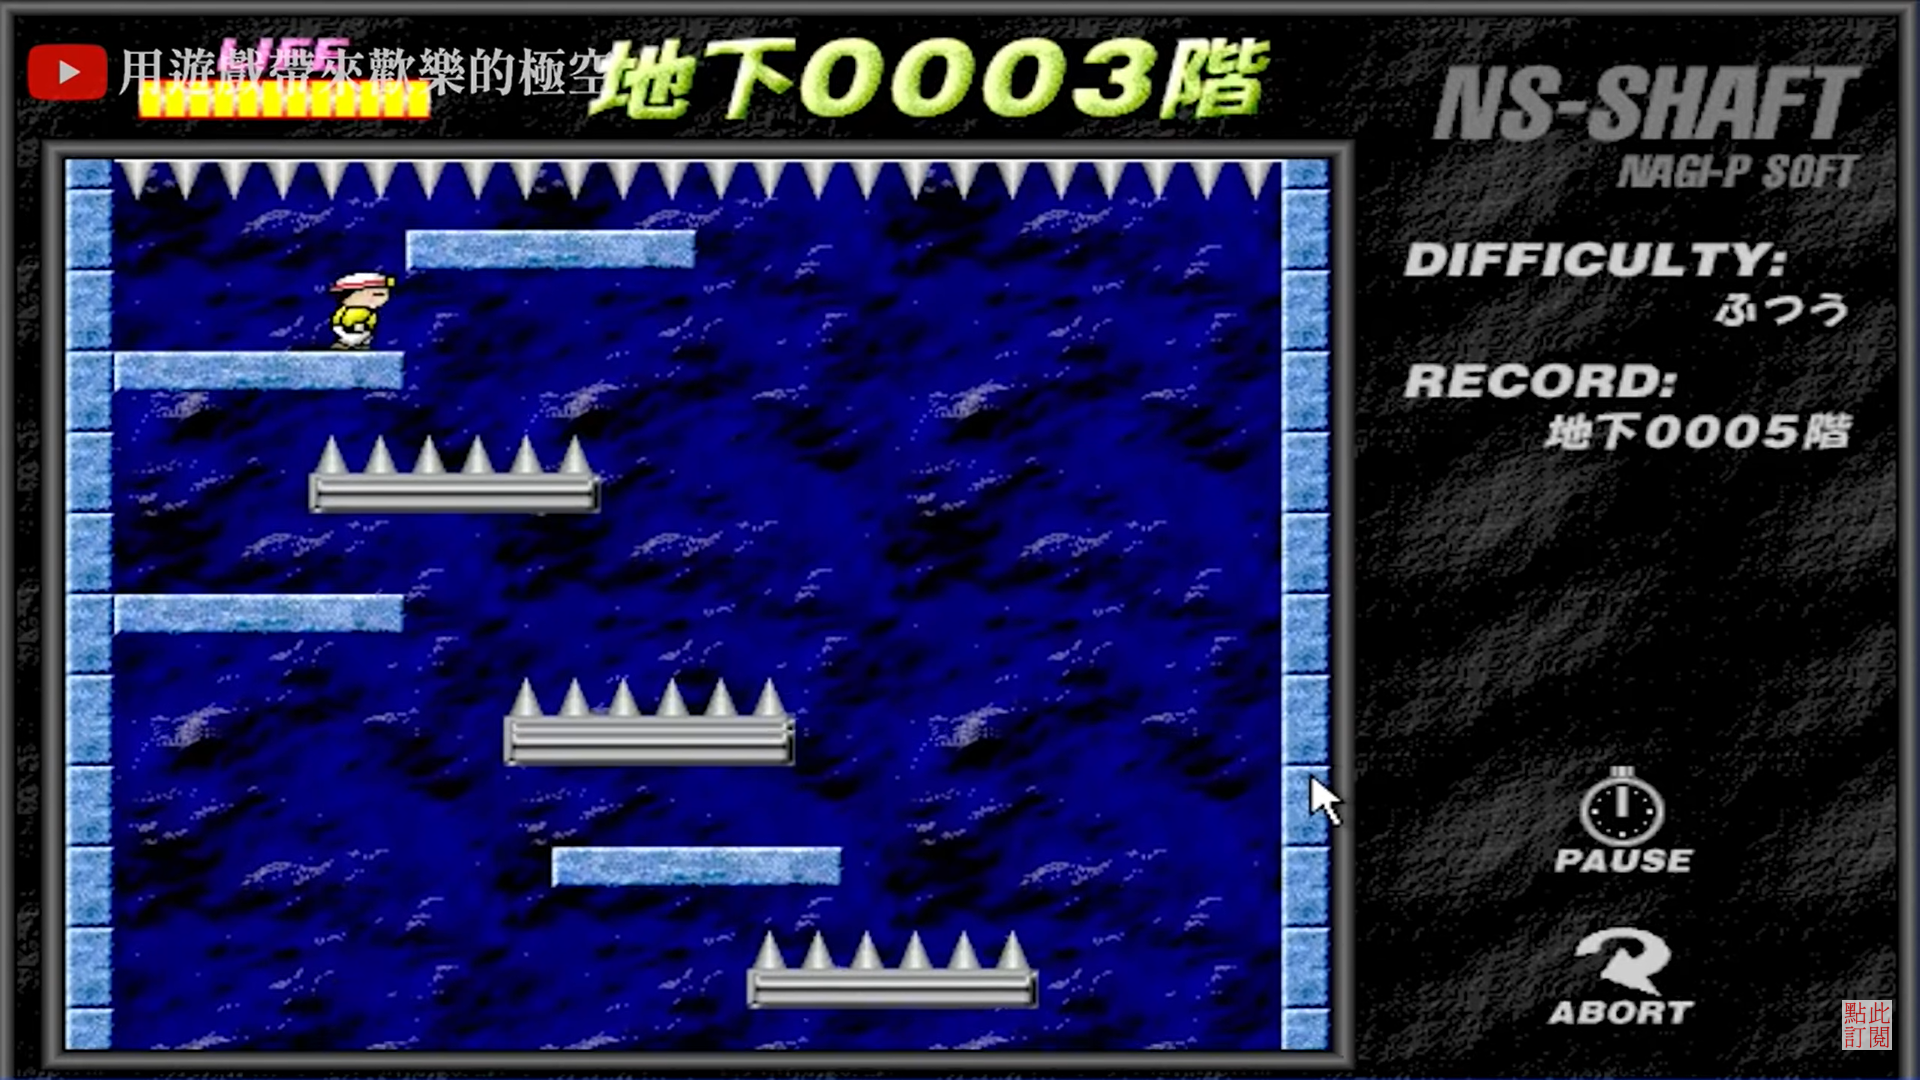
\includegraphics[width=0.75\textwidth]{NS-Shaft.png}
\caption{\label{fig:NS-Shaft}小朋友下樓梯的遊戲畫面\\Source: \protect\url{https://www.play337.com/a.asp?id=70}}
\end{figure}

% \begin{addmargin}[3em]{1em}
% \centering

% \end{addmargin}

% \end{abstract}
\newpage

\section{遊戲架構}

主程式主要由三個部分組成:起始畫面、遊戲內容、遊戲結束畫面,如Code~\ref{code:Main.jack}。可以注意到每次執行時,地圖的seed都是不同的,而且因為\texttt{Random function}會在遊戲中被多次呼叫,所以第二次玩開始,每次生成的地圖都是獨特的。

% \fontfamily{cmtt}\selectfont
% \lstinputlisting[language = Java, label={code:Main.jack}, caption = Main.jack]{Main.jack}

\begin{lstlisting}[language=java, label={code:Main.jack}, caption = Main.jack]
class Main {
    function void main() {
        var Game game;
        var bool play;
        var int point;
        var int seed;
        do Startscreen.startscreen();
        let play = true;
        let seed = 550;
        while (play){
            do Game.init();
            let game = Game.new(seed);
            let point = game.run();
            do game.dispose();
            let play = Endscreen.endscreen(point);
            let seed = LCGRandom.randRange(0, 30000);
        }
        return;
    }
}
\end{lstlisting}

\newpage
\subsection{起始畫面}
在程式執行之初,會到起始畫面。裡面有手寫的遊戲標題、操作說明(左鍵向左移、右鍵向右移)。「\~{} Press any button to start \~{}」的字樣會閃爍,提示玩家可以按任意鍵開始遊戲。如圖\ref{fig:GameImage_Startscreen}

\begin{figure}[H]
\centering
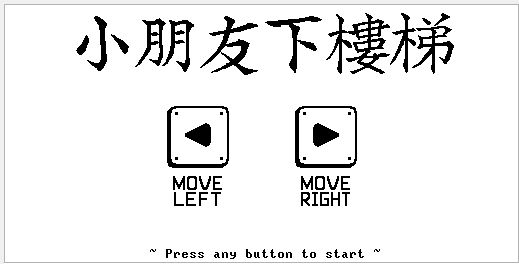
\includegraphics[width=0.65\textwidth]{GameImage_Startscreen.png}
\caption{\label{fig:GameImage_Startscreen}起始畫面}
\end{figure}

\subsection{主遊戲}
當玩家按下任意鍵,遊戲就會開始,遊戲介面如圖\ref{fig:GameImage_map}。

遊戲介面分成兩塊,左半邊為遊戲內容,右半邊則為血量、分數(層數),運作方式如下:

\begin{itemize}
\item 血量:滿血有12血,碰到上方尖刺扣4血,站於尖刺樓梯上扣2血,站於正常樓梯上補1血,掉落虛空中直接歸0。
\item 分數:每當小朋友掉落一段距離,分數就會增加,玩家的目標就是要保持小朋友活著,盡量的往下掉。
\end{itemize}

小朋友一開始保證站在最上方、正中央的階梯上。
隨著樓梯不斷上升,玩家可以用左右鍵控制小朋友左右移動而向下掉落。
小朋友的血量為0的同時,遊戲也會結束。

\begin{figure}[H]
\centering
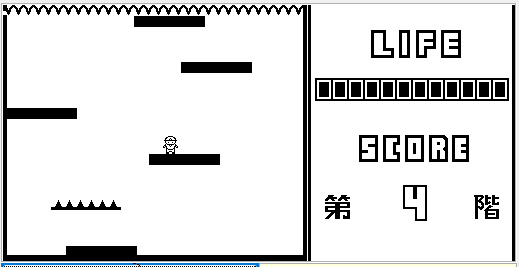
\includegraphics[width=0.65\textwidth]{GameImage_map.png}
\caption{\label{fig:GameImage_map}遊戲畫面}
\end{figure}

\newpage
大致上實作的方式如虛擬碼(Code~\ref{code:framework of the game})所示。

\begin{lstlisting}[language=java, caption={the framework of the game},label=code:framework of the game]
while (HP > 0){
    //move
    if (Left is pressed) {
        let the child take a step to the left;
    } else if (Right is pressed) {
        let the child take a step to the right;
    }
    
    //Fall
    if (stand on a stair) {
        let the child be rised with the stair;
        if (the stair the child standing on is spikes){
            HP = HP - 2;
        } else if (HP < 12) {
            HP = HP + 1;
        }
        if (the child touched the top spikes){
            HP = HP - 4;
            let the child fall a distance;
        }
    } else {
        let the child fall a distance;
        if (the child fall to the bottom){
            HP = HP - 12;
        }
    }
    
    //update
    rise the stairs;
    pause for a short time;
}
\end{lstlisting}


\newpage

\subsection{結束畫面}

若血量為0,遊戲就會結束,進入結束畫面。畫面中的數字為結束前玩家得到的分數(小朋友下落的距離)。小段延遲後,會有提示文字顯示出來,此時可以按左鍵離開遊戲(結束Main函式),或按右鍵重新開始。如圖\ref{fig:GameImage_Gameover}所示。

\begin{figure}[H]
\centering
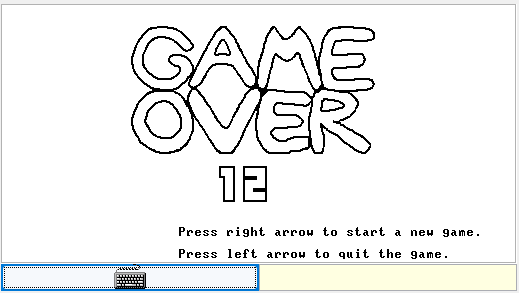
\includegraphics[width=0.65\textwidth]{GameImage_Gameover.png}
\caption{\label{fig:GameImage_Gameover}結束畫面}
\end{figure}

\section{編寫過程}

一開始我們只有定出大方向:我們要做一個遊戲。後來經過幾次討論後,決定要做小朋友下樓梯。觀察網路上查到的小朋友下樓梯版本後,我們討論出了大致的規則,並創了github repo來管理我們的程式。

但要如何開始呢?我們參考了網路上用Jack寫的跳跳鳥遊戲的主架構:\\  \url{https://github.com/N2Tstud3nt/nand2tetris-project09-Flappy-Bird}~。在成品中,我們的\texttt{Random function}及分數的大數字圖也是來自這個專案。

打好基本的程式架構後,就從\texttt{class Game}開始實作,這部分大概分成幾個小階段:

\begin{itemize}
    \setlength{\parsep}{-1em}
    \setlength{\parskip}{0em}
    \setlength{\itemsep}{-4pt}
    \item 成功生成普通階梯
    \item 畫出小朋友、可以移動小朋友、小朋友會掉落
    \item 畫出地圖(上方的尖刺、遊戲部分與統計部分分隔)、做出血量條
    \item 成功讓階梯移動、不斷生成
    \item 小朋友可以站在階梯上,並且會被扣血,但不會加血(已完成最基本遊戲)
    \item 小朋友可以被加血
    \item 新增了有尖刺的階梯
    \item 微調、修正與美化
\end{itemize}

在遊戲大致可以玩後,我們才新增了起始畫面與結束統計畫面。原本還想新增一些功能,但是程式碼幾乎到上限,只好作罷。

\section{心得}
\subsection{段蓉杉}


\subsection{洪銘德}
這是我第一次做專案,也是第一次與別人合作寫程式,當然亦是我第一次使用github。我以前幾乎都寫\texttt{C/C++},完全沒有寫過\texttt{Java},\texttt{Jack}對我是一個非常陌生的語言。從零基礎,搞不懂\texttt{function}、\texttt{method}的差別,電腦裡面沒有github很擔心自己會拖累進度,到後來可以很順的寫出自己想要的遊戲、順利用git合作,超級讓我有成就感的。

在製作的過程中,畫圖也占了一大份時間,像是結束畫面的GAMEOVER,我就畫了三、四個小時,開始畫面的標題「小朋友下樓梯」是我的自信作,這也花我很多時間,但我覺得超好看的!

在這份專案中,我認識到變數命名的重要性,蓉杉寫的部分命名都很清楚,還會註解寫功能,讓我在看的時候很快就能理解;而我的命名就比較亂(我有盡量讓自己的code比較清楚了),所以就沒那麼好理解。

我也學到,溝通、建立共識、良好分工真的很重要。在以前的報告中,我習慣默默做、然後期望組員也會自己做事,自己有做事也不太會去講,但這在共同專案是不可行的,不應該有一些沒有根據的假設,像是遊戲架構、想像,應該直接講清楚,並且在做事前就跟對方說好自己要做什麼,在實做的時候才會比較有方向、不會與對方衝突。

很感謝蓉杉,他真的是一個超級棒的組員,我們都很主動的做事,在對方比較忙時也會互相cover,兩人對這個專案的貢獻都是不可或缺的。

\newpage
\section{分工}
參考Github的commit紀錄,並列出主要項目:
\begin{itemize}
    \setlength{\parsep}{-1em}
    \setlength{\parskip}{0em}
    \setlength{\itemsep}{-4pt}
    \addtolength{\itemindent}{4em}
    \item[11/31   ] 基本程式架構
    \item[11/31 蓉杉] 階梯生成
    \item[12/01   ] 討論遊戲雛形、規則
    \item[12/02 蓉杉] 小朋友掉落、按鍵移動
    \item[12/03 銘德] 畫出地圖(上方的尖刺、遊戲部分與統計部分分隔)、做出血量條
    \item[12/04 銘德] 階梯可以移動、不斷生成
    \item[12/06 銘德] 小朋友可以站在階梯,與階梯一同向上,但判定並不穩定
    \item[12/06 銘德] 小朋友會被扣血,但不會加血(已完成最基本遊戲)
    \item[12/19 蓉杉] 小朋友掉到一般階梯上時會被治癒
    \item[12/19 蓉杉] 新增尖刺樓梯
    \item[12/22 蓉杉] 重畫(縮小)小朋友,使動畫可以更流暢
    \item[12/22 蓉杉] 修正小朋友的位置判定,使他可以好好地站在樓梯上
    \item[12/24 蓉杉] 美化地圖、新增LIFE、SCORE、第層字樣
    \item[12/24 銘德] 新增計分
    \item[12/25 銘德] 新增起始畫面
    \item[12/26 銘德] 新增結束畫面
    \item[12/26   ] 程式長度幾乎達到上限
    \item[12/27 銘德] 期末報告製作
\end{itemize}

% \section{References}
\section{參考資料}
\begin{itemize}
\item[1] nand2tetris-project09-Flappy-Bird\\ \url{https://github.com/N2Tstud3nt/nand2tetris-project09-Flappy-Bird}
\item[2] \LaTeX ~Template: Final Project Report\\ \url{https://www.overleaf.com/articles/final-project-report/nmgqcbxrrhcc}
\item[3] Wiki: NS-SHAFT\\
\url{https://zh.wikipedia.org/zh-tw/NS-SHAFT}
\end{itemize}

% \noindent\rule{18.5cm}{0.4pt}
\end{document}